\frame{
\large
\begin{enumerate}
\setcounter{enumi}{2}
 \item Marco metodológico.
  \begin{itemize}
  \item Metodología de la Investigación.
  \item Definición del Ciclo de Vida para Datos Enlazados Abiertos.
  \item Aplicación del Ciclo de Vida al \textit{e-Procurement}.
  \item Creación del sistema MOLDEAS.
  \end{itemize}

\end{enumerate}

}


\frame{
  \frametitle{Metodología de la Investigación}

\begin{block}{Tipo}<1->
Investigación cuantitativa con base en evidencias empíricas.
Carácter descriptivo y comparativo.
\end{block}
\begin{exampleblock}{Diseño}<2->
\begin{enumerate}
 \item Definición Ciclo de Vida de Datos Enlazados Abiertos.
\item  Aplicación al dominio de \eproc.
\item  Creación del sistema MOLDEAS.
\item  Definición y ejecución de experimentos.
\end{enumerate}
\end{exampleblock}
}


\frame{
  \frametitle{Metodología de la Investigación}
\begin{alertblock}{Universo de Estudio}
Tres principales conjuntos de datos seleccionados:
\begin{enumerate}
\item Datos de anuncios de licitación (1 Millón) provistos por Euroalert.net desde 2008 a 2011.
\item Catálogos de Clasificaciones de Productos y Servicios (9: CPV, CPA, NAICS, etc.) provistos por UE, ONU, EEUU, etc.
\item Organizaciones, personas y países (clasificación NUTS de la UE).
\end{enumerate}
\end{alertblock}
}

\subsection*{Definición del Ciclo de Vida para Datos Enlazados Abiertos}

\frame{
  \frametitle{Visión General} 

\begin{figure}[htb]
\centering
  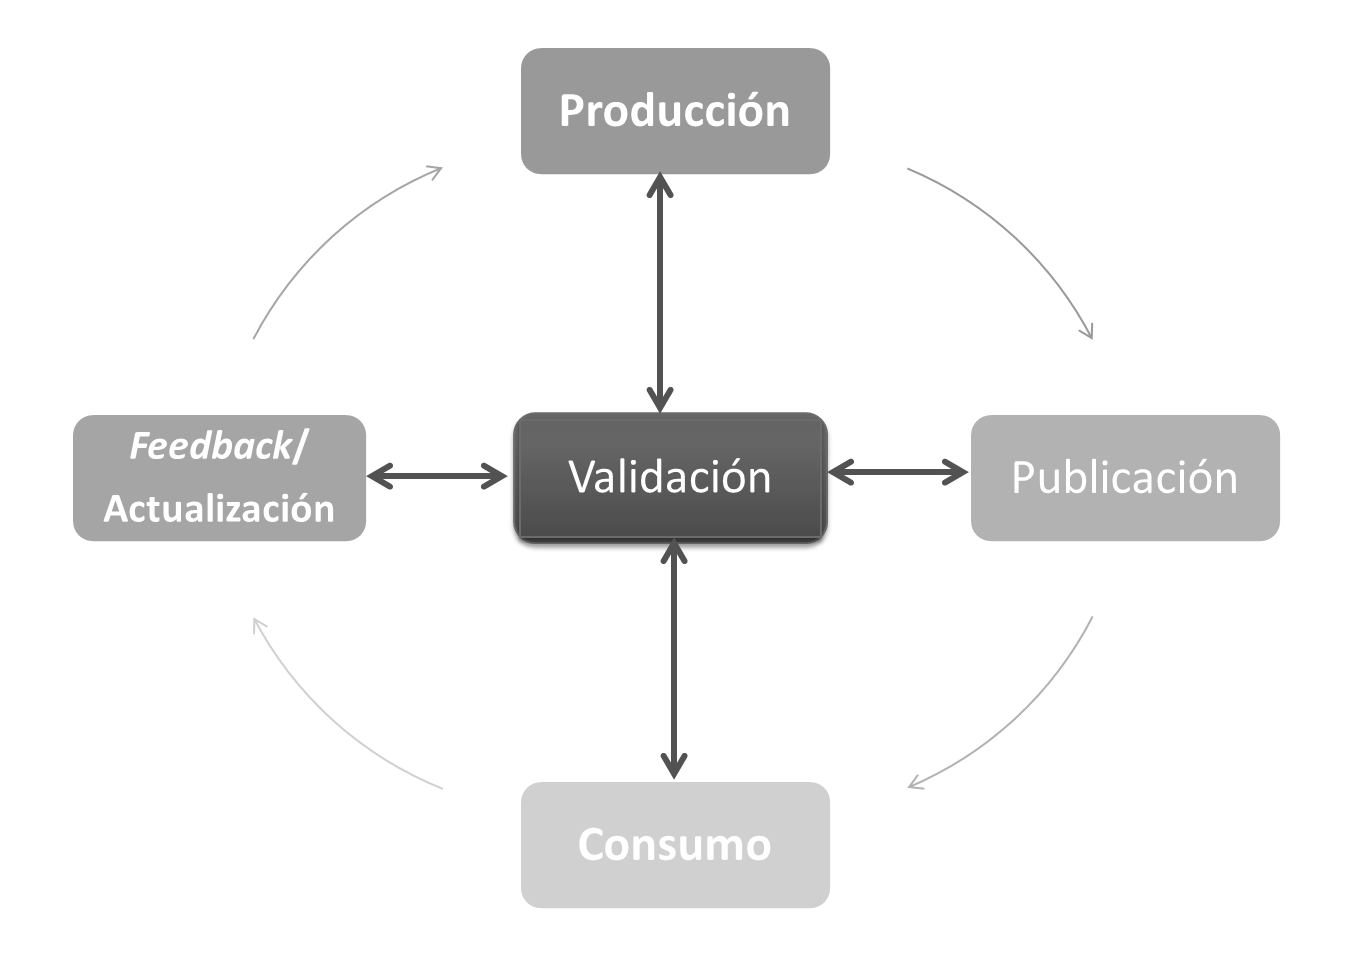
\includegraphics[width=8cm]{imgs/lld}
\caption{Procesos del Ciclo de Vida de Datos Enlazados Abiertos.}
\end{figure}

}


% 
% \frame{
%   \frametitle{Definiciones}
% 
% \begin{block}{Proceso $p$}<1->
% Se define un proceso $p$, como la aplicación de uno o varios métodos semánticos. 
% \end{block}
% 
% 
% \begin{exampleblock}{Método Semántico $sm$}<2->
% Se define un método semántico $sm$, como la consecución de $n$ tareas para llevar a cabo
% una operación sobre un \dataset. 
% 
% {\tiny El \dataset puede ser un conjunto de valores y datos $\mathcal{G}$, o bien
% un \dataset RDF, $\mathcal{D}$, dependiendo del proceso.}
% \end{exampleblock}
% 
% 
% \begin{alertblock}{Tarea $t$}<3->
%  Es cada uno de los pasos que se han de llevar a cabo para realizar un método semántico.
% \end{alertblock}
% 
% }



% \frame{
%   \frametitle{Proceso de Producción} 
% \begin{block}{Método Semántico de Producción}
% $SPM$ es una función que para un conjunto de tuplas de entrada o \dataset $\mathcal{G}$ y un conjunto de \textit{mapeos} $\mathcal{M}$  
% genera un \dataset RDF $\mathcal{D}$.
% \end{block}
% \begin{center}
%     $SPM : \mathcal{G} \times \mathcal{M} \longrightarrow \mathcal{D}$
% \end{center}
% 
% \begin{itemize}
%  \item Para todo valor $g_{i}$ del conjunto de entrada $\mathcal{G}$, existe al menos un
% \textit{mapeo} $m_{i}$ en el conjunto $\mathcal{M}$.
% \end{itemize}
% 
% }

% \frame{
%   \frametitle{Proceso de Publicación} 
% 
% \begin{block}{Método Semántico de Publicación}
% $S\mathcal{P}M$ es una función que para un \dataset RDF $\mathcal{D}$ y un conjunto de características
% de publicación $\mathcal{P}$, obtiene como resultado un \dataset RDF $\mathcal{D}_{pub}$ publicado cumpliendo $\mathcal{P}$.
% \end{block}
% 
% \begin{center}
%     $S\mathcal{P}M :  \mathcal{D} \times \mathcal{P} \longrightarrow \mathcal{D}_{pub}$
% \end{center}
% Las características contenidas en esta definición de un $S\mathcal{P}M$ son las siguientes:
% \begin{itemize}
%  \item $\mathcal{D} \approxeq \mathcal{D}_{pub}$, ya que se pueden utilizar técnicas para
% filtrar ciertos datos presentes en $\mathcal{D}$.
%  \item El conjunto de características de publicación $\mathcal{P}$ se utilizan para la validación
% de $\mathcal{D}_{pub}$.
%  \end{itemize}
% 
% }

% \frame{
%   \frametitle{Proceso de Consumo} 
% 
% \begin{block}{Método Semántico de Consumo}
% $SCM$ es una función que para un \dataset RDF $\mathcal{D}_{pub}$, con unas características de publicación $\mathcal{P}$ y un conjunto de \textit{mapeos}
% $\mathcal{M}^1$, obtiene como resultado la representación de los recursos $r_k \in \mathcal{D}_{pub}$ en otro modelo formal.
% \end{block}
% 
% \begin{center}
%     $SCM :  \mathcal{D}_{pub} \times \mathcal{M}^1 \longrightarrow \mathcal{D}_{consum}$
% \end{center}
% Las características que tiene esta definición de un $SCM$ son las siguientes:
% \begin{itemize}
%  \item $\mathcal{D}_{pub}$ no es modificado por los métodos de consumo.
%  \item $\mathcal{P}$ indica como se accede al \dataset RDF.
%  \item $\mathcal{M}^1$ indica como transformar el \dataset $\mathcal{D}_{pub}$ a la representación objetivo.
%  \end{itemize}
% 
% }

% \frame{
%   \frametitle{Proceso de Validación} 
% 
% \begin{block}{Método Semántico de Validación}
% $SVM$ es una función que para un \dataset RDF $\mathcal{D}$ y un conjunto de características
% a validar $\mathcal{V}$, obtiene como resultado un conjunto de aserciones $\mathcal{A}$.
% \end{block}
% 
% \begin{center}
%     $SVM :  \mathcal{D} \times \mathcal{V} \longrightarrow \mathcal{A}$
% \end{center}
% Las características que tiene esta definición de un $S\mathcal{P}M$  son las siguientes:
% \begin{itemize}
%  \item El \dataset RDF $\mathcal{D}$ no es modificado durante el proceso de validación.
%  \item El conjunto de características a validar $\mathcal{V}$ depende del proceso a contrastar.
%  \item El conjunto de aserciones obtenidas tras el proceso de validación $\mathcal{A}$, indica el grado de cumplimiento de $\mathcal{D}$ de acuerdo a $\mathcal{V}$.
%  \end{itemize}
% 
% }


% \frame{
%   \frametitle{Proceso de Realimentación} 
% 
% \begin{block}{Método Semántico de Realimentación}
% $SFM$ es una función que para un \dataset RDF $\mathcal{D}$ publicado como $\mathcal{D}_{pub}$ y un conjunto de relaciones y 
% valores a modificar $\mathcal{RV}$, obtiene como resultado un nuevo \dataset RDF $\mathcal{D}'$ que se publica como $\mathcal{D}'_{pub}$.
% \end{block}
% 
% \begin{center}
%     $SFM :  \mathcal{D}_{pub} \times \mathcal{RV} \longrightarrow \mathcal{D}'$
% \end{center}
% 
% 
% 
% }

% \frame{
%   \frametitle{Proceso de Realimentación} 
% \begin{itemize}
%  \item El \dataset RDF publicado $\mathcal{D}'$, se considera un nuevo conjunto
% de datos diferente a $\mathcal{D}_{pub}$.
%  \item El \dataset RDF $\mathcal{D}$, sólo se modifica en la parte de datos
% que se haya publicado como $\mathcal{D}_{pub}$. En muchos casos: $\mathcal{D}_{pub} \approxeq \mathcal{D}$.
%  \item El conjunto de relaciones y valores a modificar $\mathcal{RV}$ es un conjunto de tripletas
% de la forma $<r_k,p,v>$, donde $r_k$ es un recurso del \dataset $\mathcal{D}_{pub}$, $p$ es una relación
% presente en el recurso $r_k$ y $v$ es el valor de la relación $p$ en $r_k$. 
%  \item Los cambios en los valores de las tripletas de un recurso pueden implicar cambios en el modelo
% formal $\mathcal{O}$ de los recursos.
%  \end{itemize}
% }

% \frame{
%   \frametitle{Composición del Proceso de Realimentación} 
% 
% Asumiendo que:
% \begin{itemize}
%  \item $\mathcal{M}$ es el conjunto de \textit{mapeos} para la producción de un \dataset.
%  \item $\mathcal{P}$ es el  conjunto de características de publicación.
%  \item $\mathcal{M}^1$ es el conjunto de \textit{mapeos} para el consumo de datos.
%  \item $\mathcal{M}^1 = \mathcal{RV} $.
%  \item $\mathcal{D}'_{pub}$ es el \dataset RDF $\mathcal{D}'$ publicado, tras aplicar el método de realimentación.
% \end{itemize}
% 
% \begin{align}
% S\mathcal{P}M \circ SPM \circ SCM (\mathcal{D}_{pub}, \mathcal{RV}) \equiv \mathcal{D}'_{pub} \\
% S\mathcal{P}M \circ SPM \circ SCM (\mathcal{D}_{pub}, \mathcal{M}^1) \equiv \mathcal{D}'_{pub} \\
% S\mathcal{P}M \circ SPM (\mathcal{D}_{consum}, \mathcal{M}) \equiv \mathcal{D}'_{pub} \\
% S\mathcal{P}M (\mathcal{D}', \mathcal{P}) \equiv \mathcal{D}'_{pub} \\
% \mathcal{D}'_{pub} \equiv \mathcal{D}'_{pub}
% \end{align}
% 
% }


\frame{
  \frametitle{Visión Detallada-Procesos y Métodos} 

\begin{figure}[htb]
\centering
	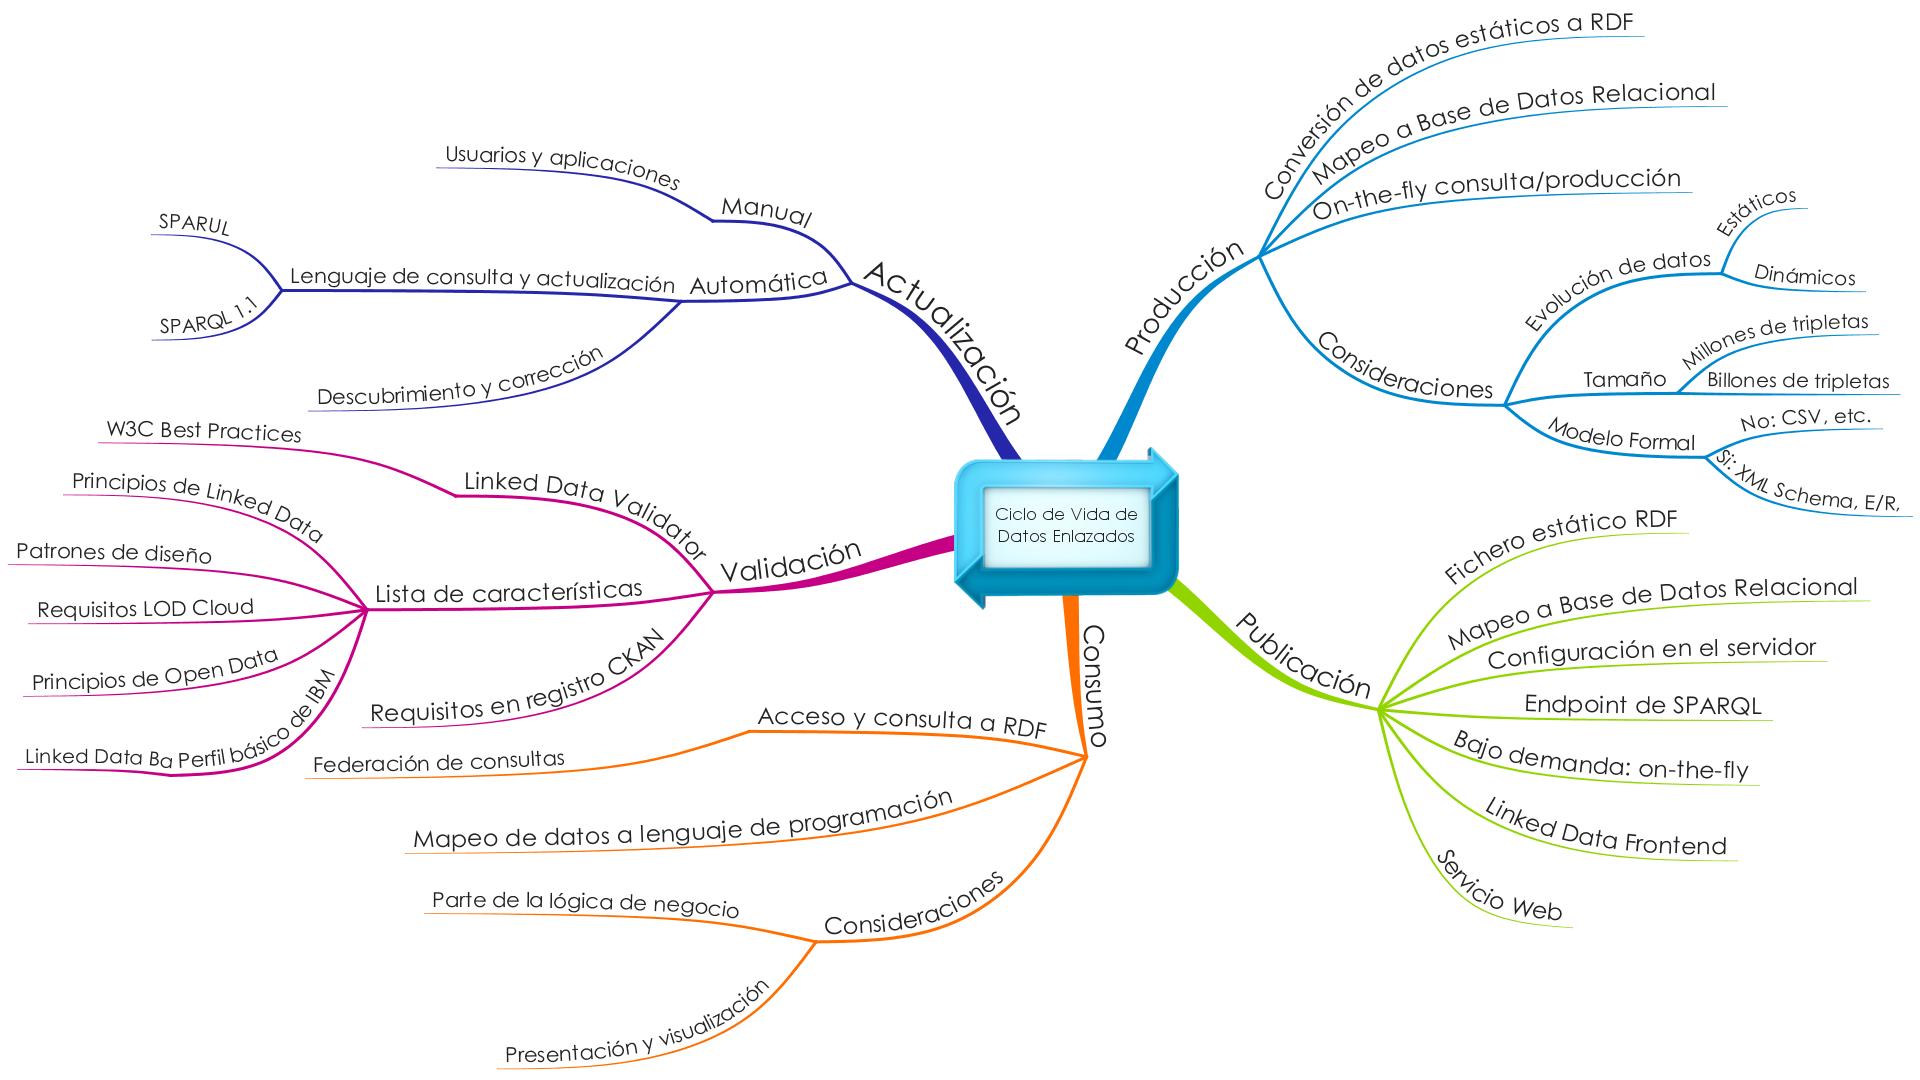
\includegraphics[width=11cm]{imgs/lld2}
\end{figure}

}

% \frame{
%   \frametitle{Listado de Tareas} 
% \scriptsize
% \begin{tabular}{lp{5.5cm}p{4cm}}
% \hline
% \rowcolor{ColorEncabezadoTabla}
% ID & Tarea & Resultado\\
% \hline
% \rowcolor{ColorFila1}
% $t_1$ & Análisis del \dataset a transformar& Especificación inicial\\
% \rowcolor{ColorFila2}
% $t_2$ & Limpieza de datos & Conjunto de datos ``limpios''\\
% \rowcolor{ColorFila1}
% $t_3$ & Selección de Vocabularios & Catálogo de vocabularios\\
% \rowcolor{ColorFila2}
% $t_4$ & Selección de otros \datasets RDF & Catálogo de 
% \datasets RDF\\
% \rowcolor{ColorFila1}
% $t_5$ & Modelado de datos en RDF & Ontología de dominio $\mathcal{O}$ y \dataset RDF $\mathcal{D}$ \\
% \rowcolor{ColorFila2}
% $t_6$ & Diseño de un Esquema de URIs & Catálogo de URIs y \dataset RDF $\mathcal{D}$ \\
% \rowcolor{ColorFila1}
% $t_7$ & Diseño Plantilla Objetivo del Recurso RDF & Plantilla recurso RDF \\
% \rowcolor{ColorFila2}
% $t_8$ & Enriquecimiento de los datos en RDF & \textit{Datasets} RDF enriquecidos\\
% \hline
% \end{tabular}  
% 
% }
% 
% \frame{
%   \frametitle{Listado de Tareas} 
% \scriptsize
% \begin{tabular}{lp{5.5cm}p{4cm}}
% \hline
% \rowcolor{ColorEncabezadoTabla}
% ID & Tarea & Resultado\\
% \hline
% \rowcolor{ColorFila1}
% $t_9$ & Transformación de los datos a RDF &$\mathcal{D}$\\
% \rowcolor{ColorFila2}
% $t_{10}$ & Reconciliación de Entidades  &Conjunto $EM$ de tuplas RDF ponderadas\\
% \rowcolor{ColorFila1}
% $t_{11}$ & Ponderación de Recursos RDF& Conjunto de tuplas $M$ de tuplas $<r_{RDF}, k>$\\
% \rowcolor{ColorFila2}
% $t_{12}$ & Validación de Recursos RDF& Tablas de grado de cumplimiento\\
% \rowcolor{ColorFila1}
% $t_{13}$ &Consolidación de datos RDF &$\mathcal{D}$ consolidado \\
% \rowcolor{ColorFila2}
% $t_{14}$ &Infraestructura para \linkeddata&Especificación\\
% \rowcolor{ColorFila1}
% $t_{15}$ &Acceso y formato en datos RDF & Especificación \\
% \rowcolor{ColorFila2}
% $t_{16}$ & Añadir metainformación a los recursos RDF& $\mathcal{D}$ enriquecido\\
% \rowcolor{ColorFila1}
% $t_{17}$ & Documentación extra&  Documentación del proceso\\
% \hline
% \end{tabular}  
% \linebreak
% {\tiny \textit{Ver descripción completa en el Capítulo 4, Sección 4.4.}}
% }


% 
% \frame{
%   \frametitle{División de Tareas en los Procesos} 
% 
% \begin{figure}[htb]
% \centering
% 	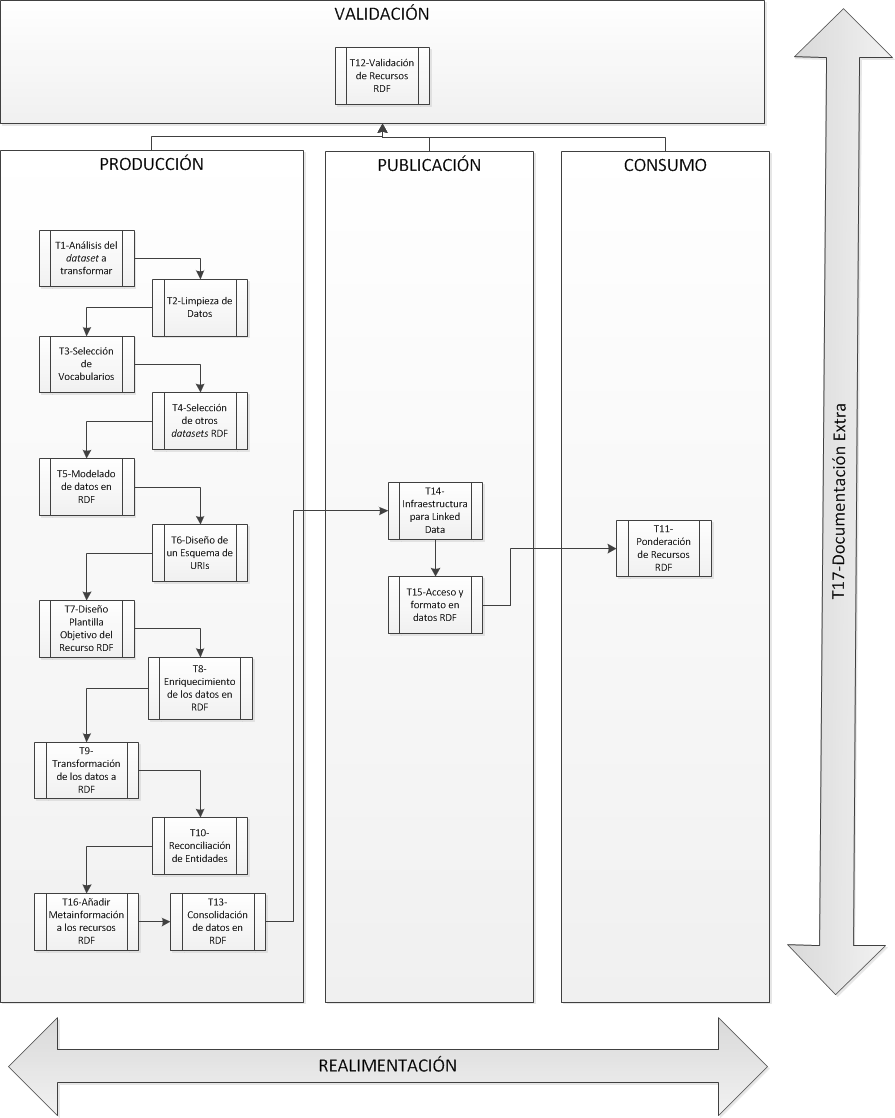
\includegraphics[width=5.8cm]{imgs/flujo-tareas}
% \end{figure}
% 
% }

\subsection*{Aplicación del Ciclo de Vida al e-Procurement}

\frame{
  \frametitle{Consideraciones Generales} 
\begin{block}{Procesos}<1->
 \begin{itemize}
 \item Métodos de Producción y Consumo dependiente del \dataset.
 \item Métodos de Publicación y Validación comunes.
\end{itemize}
\end{block}
\begin{exampleblock}{Conjuntos de Datos}<2->
\begin{itemize}
 \item Anuncios de licitación (PPN).
 \item Clasificaciones estándar de productos y servicios (PSCs).
 \item Organizaciones, personas y países.
\end{itemize} 
\end{exampleblock}

}


\frame{
  \frametitle{Métodos Aplicados} 
\begin{block}{Producción}<1->
Transformación de datos estáticos a RDF.
\end{block}
\begin{exampleblock}{Publicación}<2->
Fichero estático en RDF, \textit{Endpoint} de SPARQL y \linkeddata \textit{Frontend}.
\end{exampleblock}
\begin{alertblock}{Consumo}<3->
\textit{Mapeo} a Lenguaje de Programación.
\end{alertblock}
\begin{block}{Validación}<4->
Uso de Tablas de Validación.
\end{block}
\begin{exampleblock}{Realimentación}<5->
Actualización Ocasional.
\end{exampleblock}

}


% \frame{
%   \frametitle{Anuncios de Licitación} 
% \begin{figure}[htb]
% \centering
% 	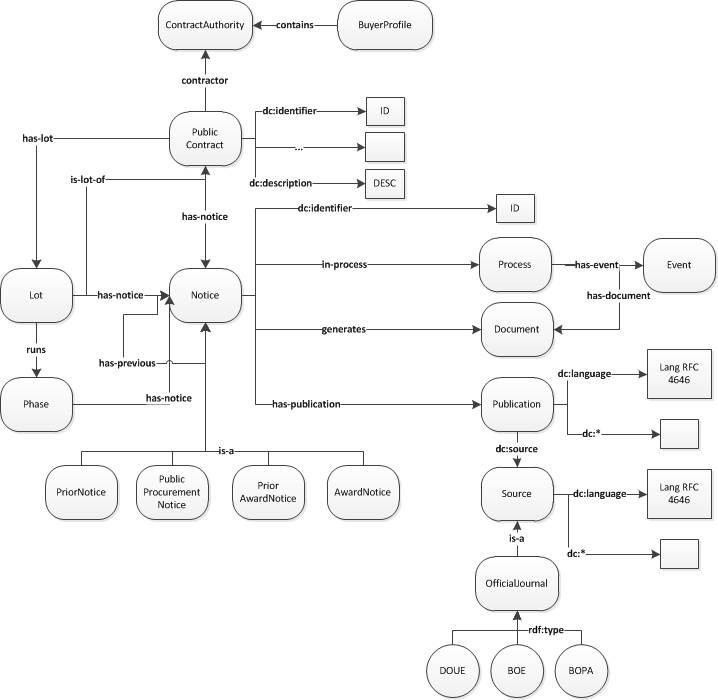
\includegraphics[width=6cm]{imgs/overview}
% \caption{Tarea $t_1$-Análisis del \dataset a transformar y Tarea $t_5$-Modelado de datos en RDF.}
% \end{figure}
% 
% }

% \frame{
%   \frametitle{Anuncios de Licitación} 
% \begin{figure}[htb]
% \centering
% 	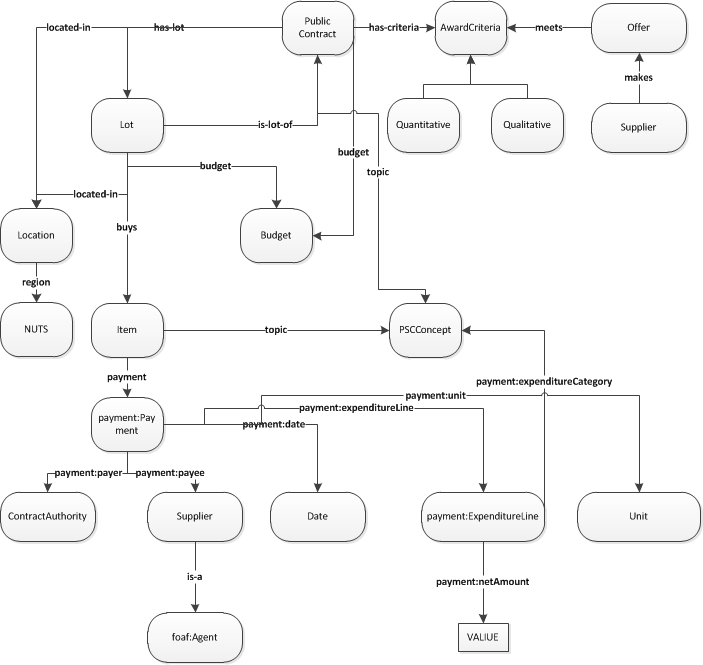
\includegraphics[width=6cm]{imgs/contract-lots}
% \caption{Tarea $t_1$-Análisis del \dataset a transformar y Tarea $t_5$-Modelado de datos en RDF (II).}
% \end{figure}
% 
% }

% \frame{
%   \frametitle{Anuncios de Licitación} 
% \begin{figure}[htb]
% \centering
% 	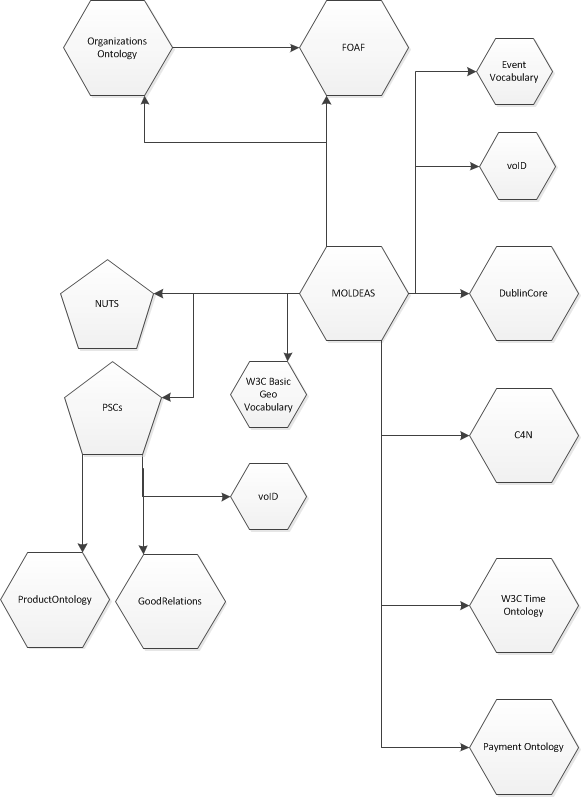
\includegraphics[width=4cm]{imgs/contract-vocabs}
% \caption{Tarea $t_3$-Selección de Vocabularios y Tarea $t_4$-Selección de otros \datasets RDF.}
% \end{figure}
% 
% }

% \frame{
%   \frametitle{Anuncios de Licitación} 
% \begin{figure}[htb]
% \centering
% 	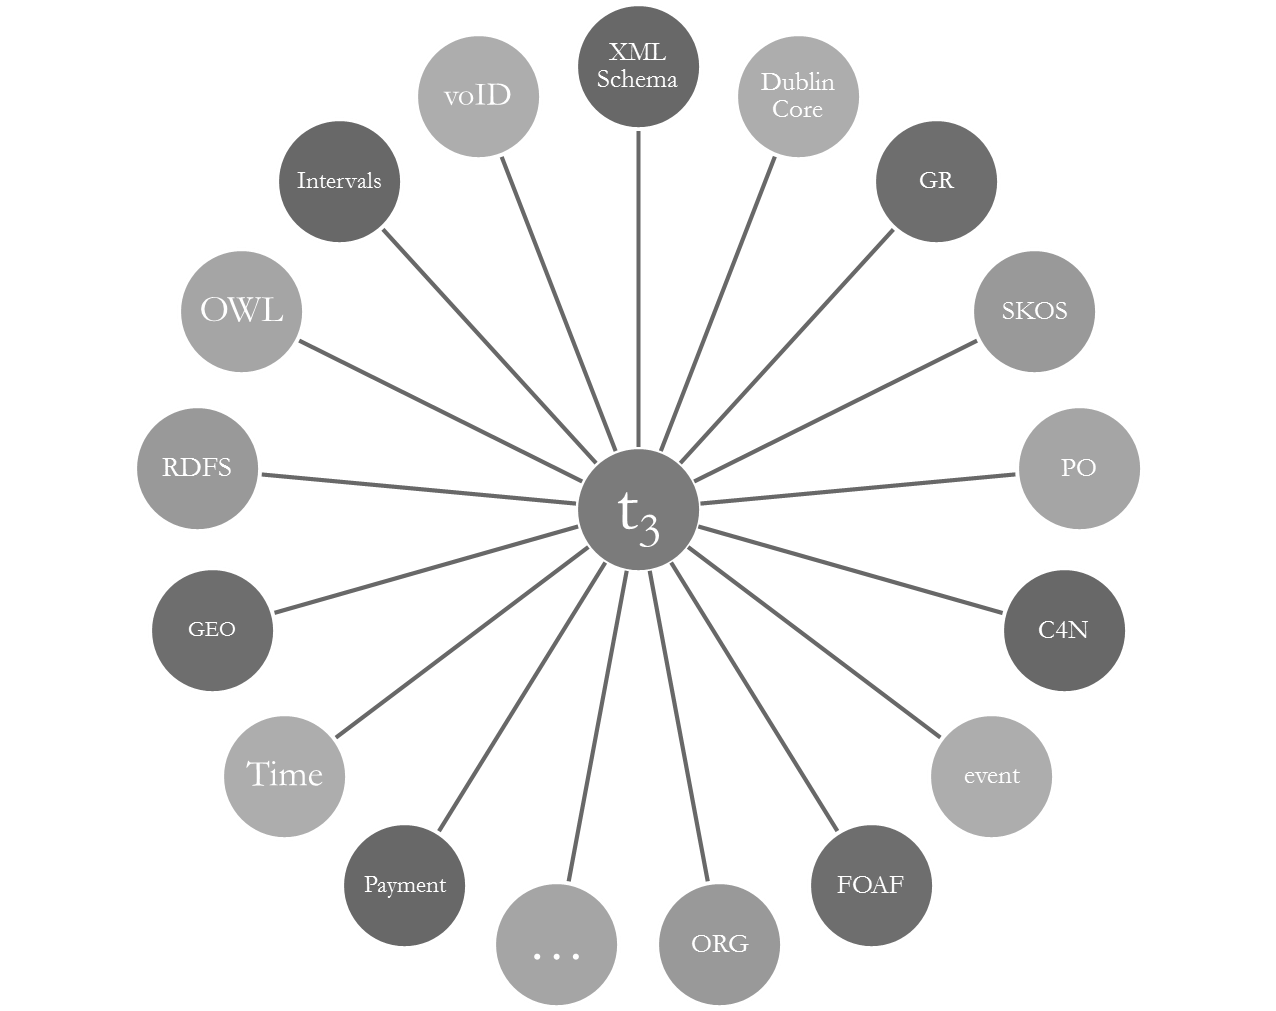
\includegraphics[width=7cm]{imgs/t3}
% \caption{Tarea $t_3$-Selección de Vocabularios.}
% \end{figure}
% 
% }

% \frame{
%   \frametitle{Anuncios de Licitación} 
% \begin{figure}[htb]
% \centering
% 	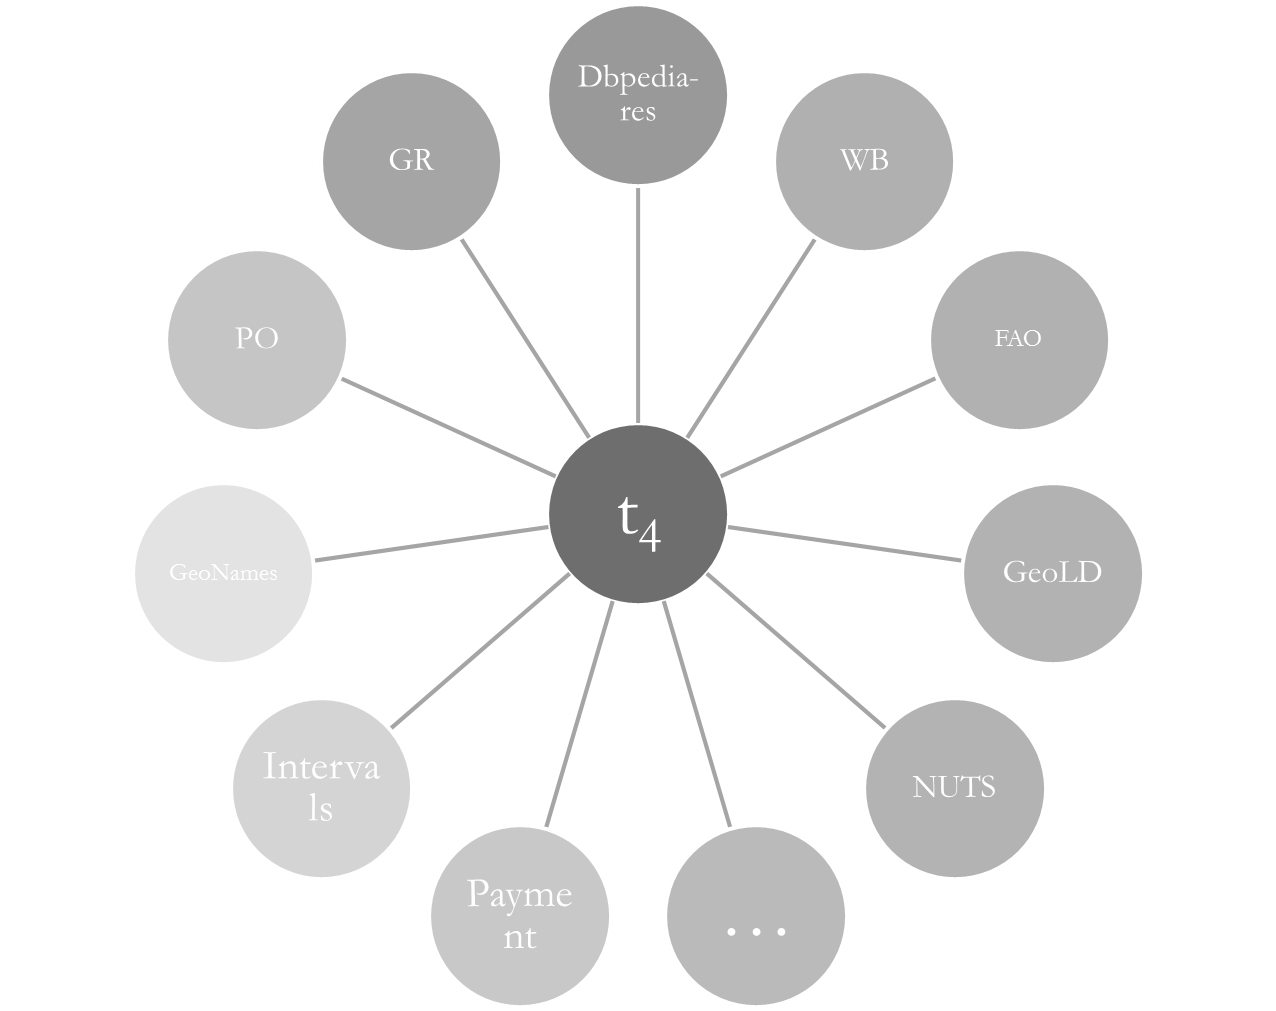
\includegraphics[width=7cm]{imgs/t4}
% \caption{Tarea $t_4$-Selección de otros \datasets RDF.}
% \end{figure}
% 
% }

% \frame{
%   \frametitle{Anuncios de Licitación} 
% \begin{block}{$t_6$-Diseño de un Esquema de URIs.}
%  \begin{itemize}
% \item \url{http://purl.org/weso/ppn/} (<base\_uri>)
% \item \url{<base_uri>/ontology} 
% \item \url{<base_uri>/{year}} 
% \item \url{<base_uri>/resource/{year}/{id}}
% \item \url{<base_uri>/resource/{year}/{id}/publication/{id}}
% \item \url{<base_uri>/resource/{year}/{id}/lot/{id}} 
% \item \url{<base_uri>/resource/{year}/{id}/lot/{id}/item/{id}} 
% \item \url{<base_uri>/resource/{year}/{id}/lot/{id}/budget}
% \item \url{<base_uri>/resource/{year}/{id}/lot/{id}/payment}
% \item \ldots
% \end{itemize}  
% \end{block}
% 
% 
% }


\frame{
  \frametitle{Resultados} 
\small
\begin{longtable}[c]{|p{4cm}|p{3cm}|p{2cm}|} 
\hline
  \textbf{Anuncios de Licitación} & \textbf{Nº de Elementos}  &  \textbf{Tripletas}  \\\hline
\endhead
PPN 2008 & $112843$  &   $677058$  \\ \hline
PPN 2009 & $399766$ &   $2398601$   \\ \hline
PPN 2009  & $431813$&  $2590880$  \\ \hline
PPN 2011 & $67044$&   $402264$   \\ \hline
\multicolumn{3}{|c|}{\textbf{Catálogo de Anuncios de Licitación} (total)} \\ \hline
PPNs & $1011466$ &  $6068803$   \\ \hline
\hline
\end{longtable}

}


% \frame{
%   \frametitle{Anuncios de Licitación} 
% \begin{figure}[htb]
% \centering
% 	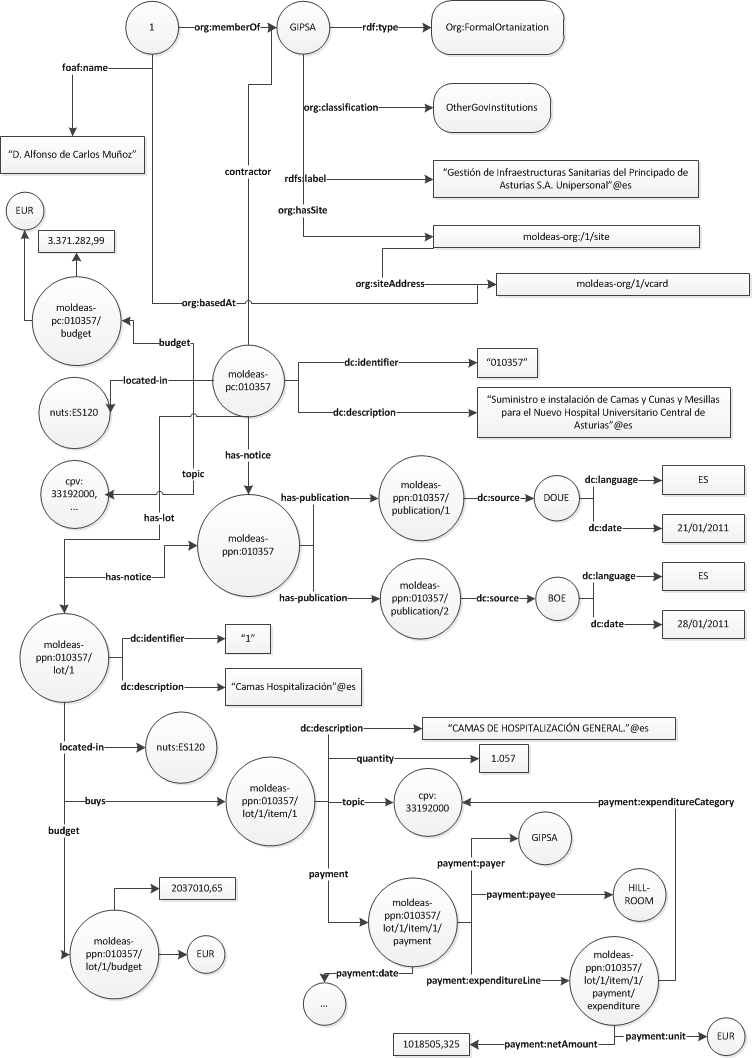
\includegraphics[width=5cm]{imgs/hospital-1}
% %\caption{Ejemplo licitación pública hospital.}
% \end{figure}
% 
% }

% \frame{
%   \frametitle{Anuncios de Licitación} 
% \begin{figure}[htb]
% \centering
% 	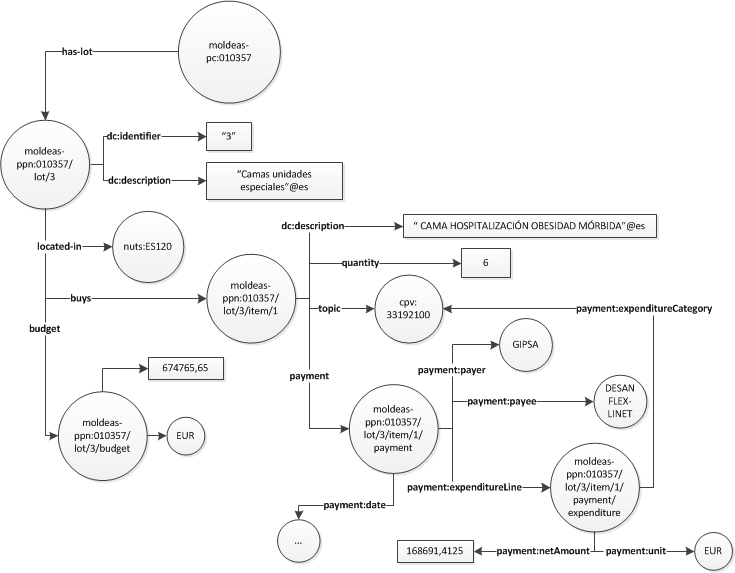
\includegraphics[width=9cm]{imgs/hospital-2}
% %\caption{Ejemplo licitación pública hospital.}
% \end{figure}
% 
% }


\frame{
  \frametitle{Clasificaciones Estándar de Productos y Servicios} 
\small
\begin{longtable}[c]{|p{6.5cm}|l|p{2cm}|} 
\hline
  \textbf{Clasificación} &  \textbf{Acrónimo} & \textbf{Organismo} \\\hline
\endhead
\textit{Common Procurement Vocabulary}, (2003 y 2008) & CPV & UE \\ \hline
\textit{Combined Nomenclature} 2012 (desde 1995) & CN & `` \\ \hline
\textit{Central Product Classification}, version 2 (2008) & CPC & \ldots\\ \hline
Clasificación de Productos por Actividad (2008) & CPA & `` \\ \hline
\textit{International Standard Industrial Classification of All Economic Activities, Rev.4} & ISIC & ONU \\ \hline
\textit{North American Industry Classification System} 2007 y 2012 & NAICS & EEUU \\ \hline
\textit{Standard International Trade Classification, Revision 4} & SITC & ONU \\ \hline
\hline
\end{longtable}

}

% \frame{
%   \frametitle{Clasificaciones Estándar de Productos y Servicios} 
% 
% \begin{enumerate}
%  \item Categorías de productos.  $Cat_{psc} = \displaystyle\bigcup_{n=0}^k{(Cat_{psc}^n)}$
% \begin{itemize}
%  \item Organización jerárquica: $Cat_{psc}^0\succ
% Cat_{psc}^1\succ...\succ Cat_{psc}^n $.
%  \item Cada elemento $t_{psc}^x$ pertenece a una, y sólo una, categoría de productos.
%   \item Categorías disjuntas: $\displaystyle\bigcap_{n=0}^k{(Cat_{psc}^n)}=\emptyset$.
% \end{itemize}
% 
% \item  Estructura taxonómica.  Cada sector es un árbol, $T_{psc}$: todos los elementos
% $t_{psc}^n$ tienen un elemento de nivel superior $t_{psc}^{n-1}$. El conjunto de sectores puede definirse como 
% un \textbf{bosque} ($\mathbb{F}_{psc}$) de árboles ($T_{psc}$):
% \begin{itemize}
%  \item $\mathbb{F}_{psc}= \displaystyle\bigcup_{m=0}^k{(T_{psc}^m)}$, con raíz $t_{psc}^0$.
%  \item Cada elemento $t_{psc}$ pertenece a uno de estos árboles de productos $T_{psc}^x$.
% \end{itemize}
%  
% \end{enumerate}
% 
% 
% }

% \frame{
%   \frametitle{Clasificaciones Estándar de Productos y Servicios} 
% \begin{figure}[htb]
% \centering
% 	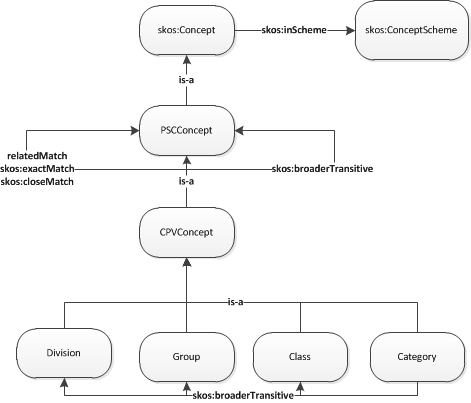
\includegraphics[width=6cm]{imgs/pscs-model}
% \caption{Tarea $t_1$-Análisis del \dataset a transformar y Tarea $t_5$-Modelado de datos en RDF.}
% \end{figure}
% 
% }

\frame{
  \frametitle{Clasificaciones Estándar de Productos y Servicios} 
\begin{figure}[!htb]
\centering
	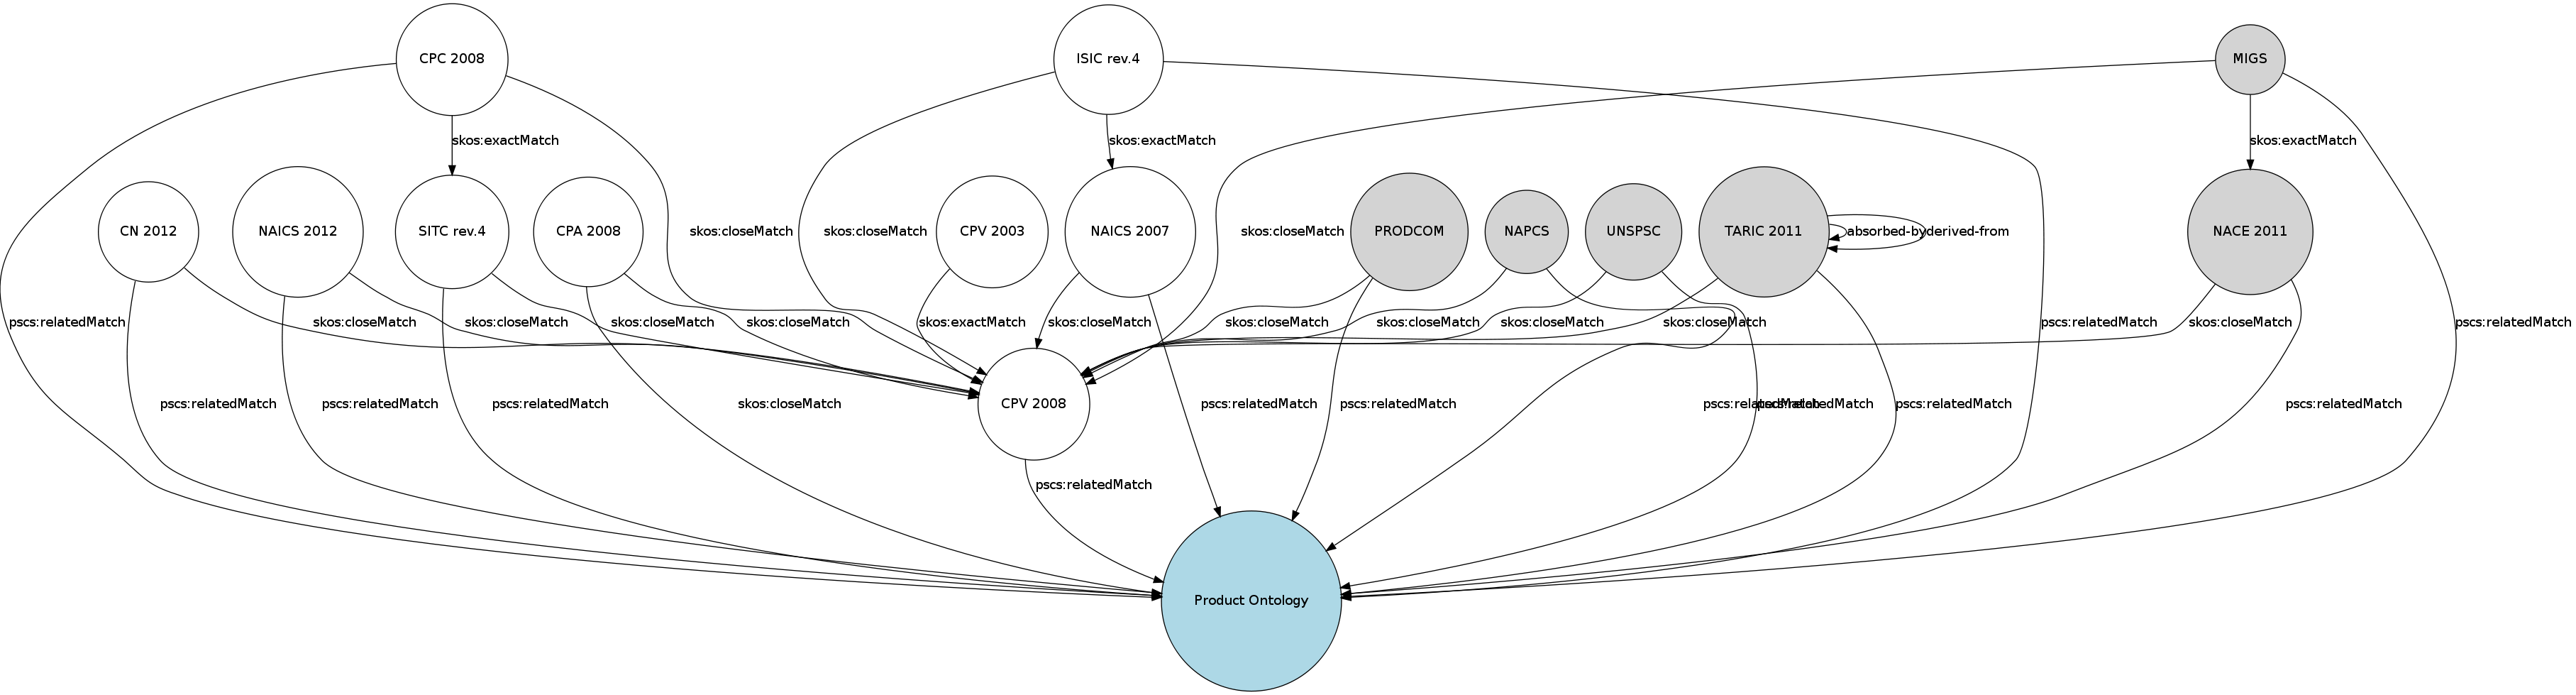
\includegraphics[width=12cm]{./imgs/pscs}
\caption{Enlaces entre las distintas Clasificaciones Estándar de Productos y Servicios.}
\end{figure}
}

% 
% \frame{
%   \frametitle{Clasificaciones Estándar de Productos y Servicios} 
% \begin{block}{$t_6$-Diseño de un Esquema de URIs.}
%  \begin{itemize}
% \item \url{http://purl.org/weso/pscs/}
% \item \url{<base_uri>/ontology}
% \item \url{<base_uri>/resource/ds}
% \item \url{<base_uri>/{psc}/{version|year}}
% \item \url{<base_uri>/{psc}/{version|year}/ontology} 
% \item \url{<base_uri>/resource/{psc}/{version|year}/{id}} 
% \item \url{<base_uri>/resource/{psc}/{version|year}/ds} 
% \end{itemize}  
% \end{block}
% 
% 
% }


\frame{
  \frametitle{Resultados-I} 
\small
\begin{longtable}[c]{|l|p{1.5cm}|p{1.8cm}|p{1.5cm}|p{2.5cm}|} 
\hline
  \textbf{PSC} & \textbf{\#}  &  \textbf{Tripletas} &  \textbf{Links} &  \textbf{Links CPV 2008} \\\hline
\endhead
CPV 2003 & $8323$  & $546135$  & $8322$ & $462$ (del CPV 2008 al 2003)   \\ \hline
CPV 2008 & $10357$ &   $803311$  & $10355$ & N/A   \\ \hline
CN 2012  & $14552$&  $137484$  & $2590$ & $2390$ \\ \hline
CPC 2008 & $4408$&   $100819$  & $4408$ & $4375$ y $1503$ (exactos)  \\ \hline
CPA 2008 & $5429$&  $92749$   & $5429$ & $5399$  \\ \hline
\multicolumn{5}{|c|}{\ldots} \\ \hline
\hline
\end{longtable}

}


\frame{
  \frametitle{Resultados-II} 
\small
\begin{longtable}[c]{|l|p{1.5cm}|p{1.8cm}|p{1.5cm}|p{2.5cm}|} 
\hline
  \textbf{PSC} & \textbf{\#}  &  \textbf{Tripletas} &  \textbf{Links} &  \textbf{Links CPV 2008} \\\hline
\endhead
ISIC v4  & $766$&  $18986$   & $766$ & $765$  \\ \hline
NAICS 2007 & $2328$&  $36292$   & $2328$ & $2300$  \\ \hline
NAICS 2012 & $2212$&  $35390$   & $2212$ & $2186$  \\ \hline
SITC v4 & $4017$&  $70887$   & $3941$ & $3811$  \\ \hline
\multicolumn{5}{|c|}{\textbf{Catálogo de Clasificaciones Estándar de Productos} (total)} \\ \hline
PSCs & $52392$ &   $1842053$ & $40351$ & $23191$  \\ \hline
\hline
\end{longtable}

}

\frame{
  \frametitle{Organizaciones, personas y países} 

\begin{figure}[htb]
\centering
	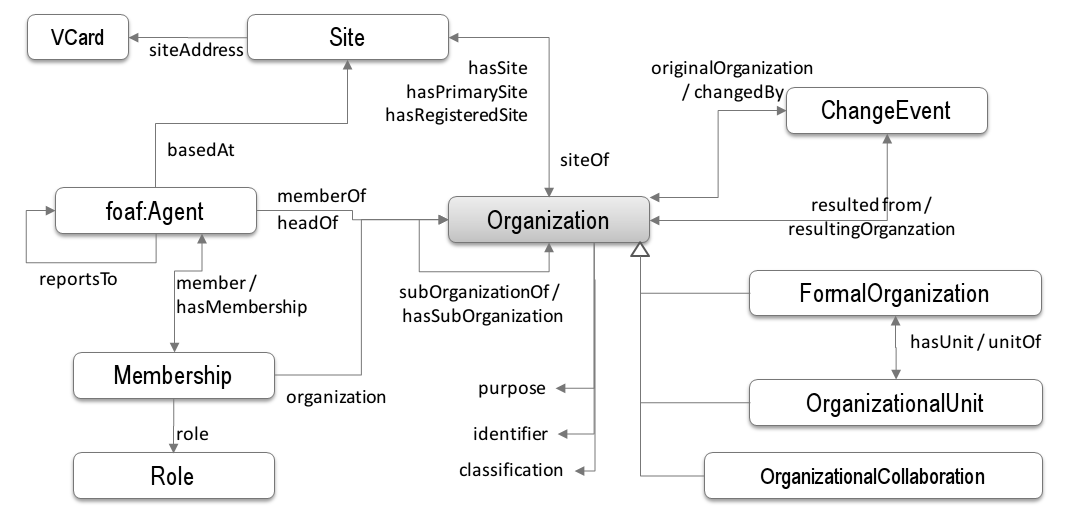
\includegraphics[width=8cm]{imgs/org}
\caption{\textit{Organizations Ontology} del W3C.}
\end{figure}

}

% \frame{
%   \frametitle{Organizaciones, personas y países} 
% \begin{block}{$t_6$-Diseño de un Esquema de URIs.}
%  \begin{itemize}
% \item \url{http://purl.org/weso/eprocurement}
% \item \url{<base_uri>/organization/ontology}
% \item \url{<base_uri>/organization/resource/ds} 
% \item \url{<base_uri>/organization/resource/{id}} 
% \item \url{<base_uri>/organization/person/resource/ds}
% \item \url{<base_uri>/organization/person/resource/{id}}
% \item \url{<base_uri>/country/ontology}
% \item \url{<base_uri>/country/resource/ds} 
% \item \url{<base_uri>/country/resource/{id}}
% \end{itemize}  
% \end{block}
% }


\frame{
  \frametitle{Resultados} 
\small
\begin{longtable}[c]{|p{2.2cm}|p{2.5cm}|p{2cm}|p{2.5cm}|} 
\hline
  \textbf{Dataset} & \textbf{\#}  &  \textbf{Tripletas} &  \textbf{Enlaces externos}  \\\hline
\endhead
Organizaciones & $50000$   & $1150020$  & $50000$ (países)   \\ \hline
Personas & $50000$    & $900219$  & $50000$  (países)  \\ \hline
Países & $246$     & $1756$  & $1779$ \\ \hline
\multicolumn{4}{|c|}{\textbf{Organizaciones, Personas y Países} (total)} \\ \hline
Agregado & $100246$  & $2051995$ & $101779$   \\ \hline
\hline
\end{longtable}

}


% \frame{
%   \frametitle{Tareas Transversales} 
% \begin{block}{Tarea $t_{12}$-Validación de Recursos RDF}
%  \begin{itemize}
%  \item Los datos RDF son correctos, ya que se ha utilizado el API de Jena.
%  \item El dominio y rango en las propiedades es correcta, la validación contra el modelo definido.
%  \item Se ha establecido metainformación sobre la procedencia a nivel de \dataset.
%  \item Todos los recursos transformados siguen la plantilla objetivo RDF.
% \end{itemize}
% \end{block}
% 
% 
% }

% \frame{
%   \frametitle{Tareas Transversales} 
% \begin{figure}[htb]
% \centering
% 	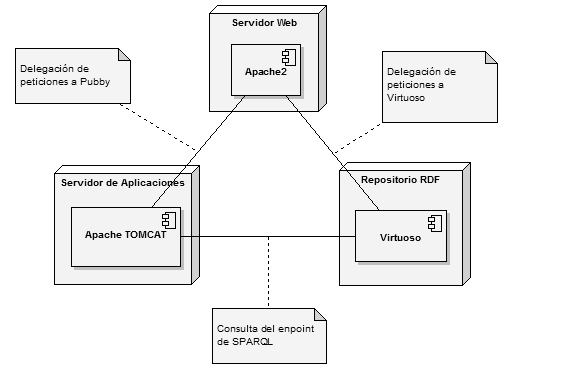
\includegraphics[width=8cm]{imgs/infra-ld}
% \caption{Tarea $t_{14}$-Infraestructura para \linkeddata.}
% \end{figure}
% 
% }

% \frame{
%   \frametitle{Tareas Transversales} 
% \small
% \begin{table}[!htb]
% \renewcommand{\arraystretch}{1.3}
% \begin{center}
% \begin{tabular}{|p{4cm}|l|p{4cm}|}
% \hline
%   \textbf{Acceso} &  \textbf{Formato} &  \textbf{Provisto por}  \\\hline
%  Petición GET    & N3/Turtle    & Apache2 \\ \hline
%  Consulta SPARQL & \textit{Spreadsheet}  & \textit{Endpoint} de SPARQL  \\ \hline
%  ``       & XML 		& ``\\ \hline
%  ``       & JSON 	& ``\\ \hline
%  ``       & Javascript 	& `` \\ \hline 
%  Consulta SPARQL y petición GET & N3/Turtle 	& \textit{Endpoint} de SPARQL y \linkeddata \textit{Frontend} \\ \hline
%  ``       & RDF/XML 	& ``\\ \hline
%  ``       & NTriples 	& `` \\ \hline
%  ``       & HTML 	& `` \\ \hline
%  \hline
%   \end{tabular}
%   \end{center}
% \caption{Tarea $t_{15}$-Acceso y formato en datos RDF.}
% \end{table} 
% }

% \frame{
%   \frametitle{Tareas Transversales} 
% \begin{block}{Tareas}
%  \begin{itemize}
%  \item $t_2$-Limpieza de datos (N/A).
%  \item $t_7$-Diseño Plantilla Objetivo del Recurso RDF (dependiente del contexto).
%  \item $t_8$-Enriquecimiento de los datos en RDF (\``).
%  \item $t_9$-Transformación de los datos a RDF.
%  \item $t_{10}$-Reconciliación de Entidades.
%  \item $t_{11}$-Ponderación de Recursos RDF.
%  \item $t_{13}$-Consolidación de datos RDF (N/A).
%  \item $t_{16}$-Añadir metainformación a los recursos RDF (\textit{voID}).
%  \item $t_{17}$-Documentación extra.
% \end{itemize}
% \end{block}
% }

\subsection*{Sistema MOLDEAS}


\frame{
  \frametitle{MOLDEAS y los procesos del Ciclo de Vida} 

\begin{figure}[htb]
\centering
	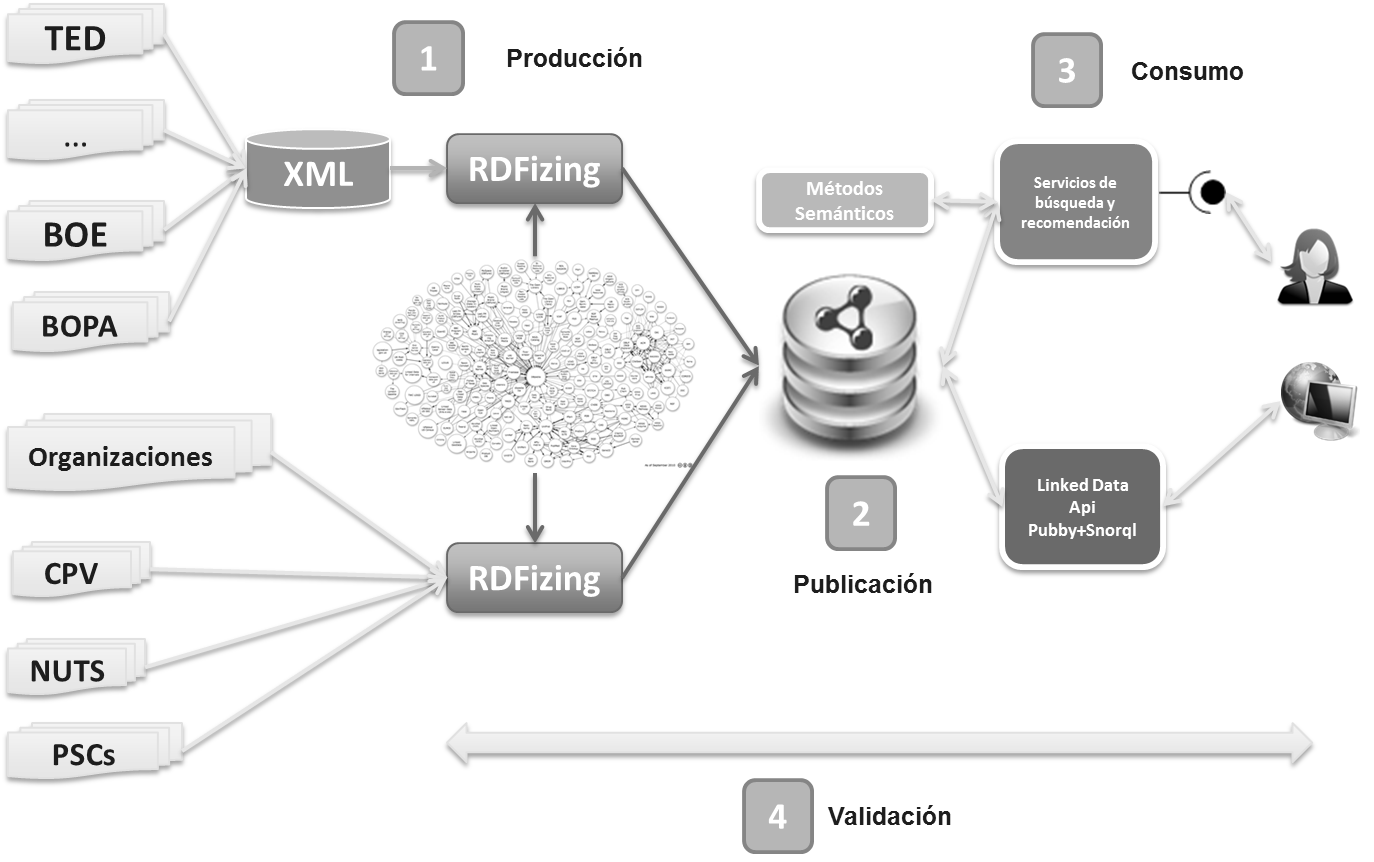
\includegraphics[width=8cm]{imgs/functional-overview}
\caption{Visión Funcional de MOLDEAS y los procesos del Ciclo de Vida de \linkeddata.}
\end{figure}
}

% \frame{
%   \frametitle{Consideraciones de Diseño} 
% \begin{block}{Buenas Prácticas}
%  \begin{itemize}
%  \item Uso de patrones de diseño: \textit{DAO, Chain of Responsibility, Adapter, TransferObject}, etc.
%  \item Aplicación por capas (Datos, Servicios, Cliente y Presentación).
%  \item Reutilización de bibliotecas existentes.
% \end{itemize}
% \end{block}
% }


% \frame{
%   \frametitle{Componentes MOLDEAS} 
% \begin{figure}[!htb]
% \centering
% 	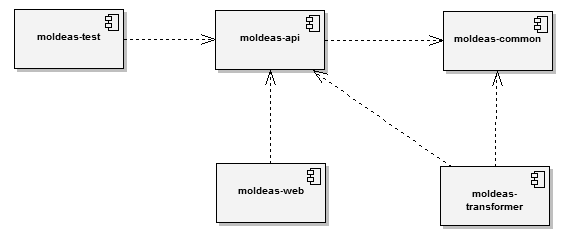
\includegraphics[width=8cm]{imgs/moldeas-componentes}
% \caption{Dependencias entre componentes en el sistema MOLDEAS.}
% \end{figure}
% }

% \frame{
%   \frametitle{Arquitectura General} 
% \begin{figure}[!htb]
% \centering
% 	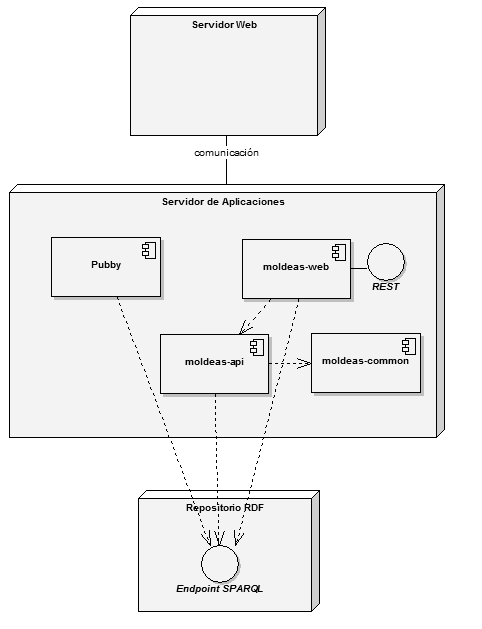
\includegraphics[width=5cm]{imgs/moldeas-despliegue}
% \caption{Diagrama de Despliegue.}
% \end{figure}
% 
% }


% \frame{
%   \frametitle{Entorno Tecnológico} 
% 
% 
% \begin{columns}[c] % the \ldotsc\ldots option specifies center vertical alignment
% \column{.5\textwidth} % column designated by a command
% 
% 
% \begin{block}{Desarrollo}<1->
%  \begin{itemize}
% \item Java 1.6.
% \item Apache Maven2.
% \item Eclipse-IDE.
% \item Repositorio Google Code.
% \item Protégé 4.1.x.
% \item Openlink Virtuoso 6.1.
% \item Google Refine y \textit{RDF extension}.
% \item \LaTeX.
% \end{itemize}
% \end{block}
% 
% 
% \column{.5\textwidth}
% 
% \begin{exampleblock}{Bibliotecas destacadas}<2->
%  \begin{itemize}
% \item Log4j 1.2.14.
% \item Junit 4.0.
% \item Apache Lucene 2.9.0.
% \item Apache Solr 1.4.1.
% \item Apache Mahout 0.4.
% \item Spring 2.5
% \item Jersey-REST 0.8.
% \item Jquery 1.4.1.
% \item Exhibit 2.2.0.
% \item Pubby 0.3.3.
% \item SNORQL.
% \end{itemize}
% \end{exampleblock}
% 
% \end{columns}
% 
% 
% }

% \frame{
%   \frametitle{Componentes: moldeas-api} 
% \begin{figure}[!htb]
% \centering
%  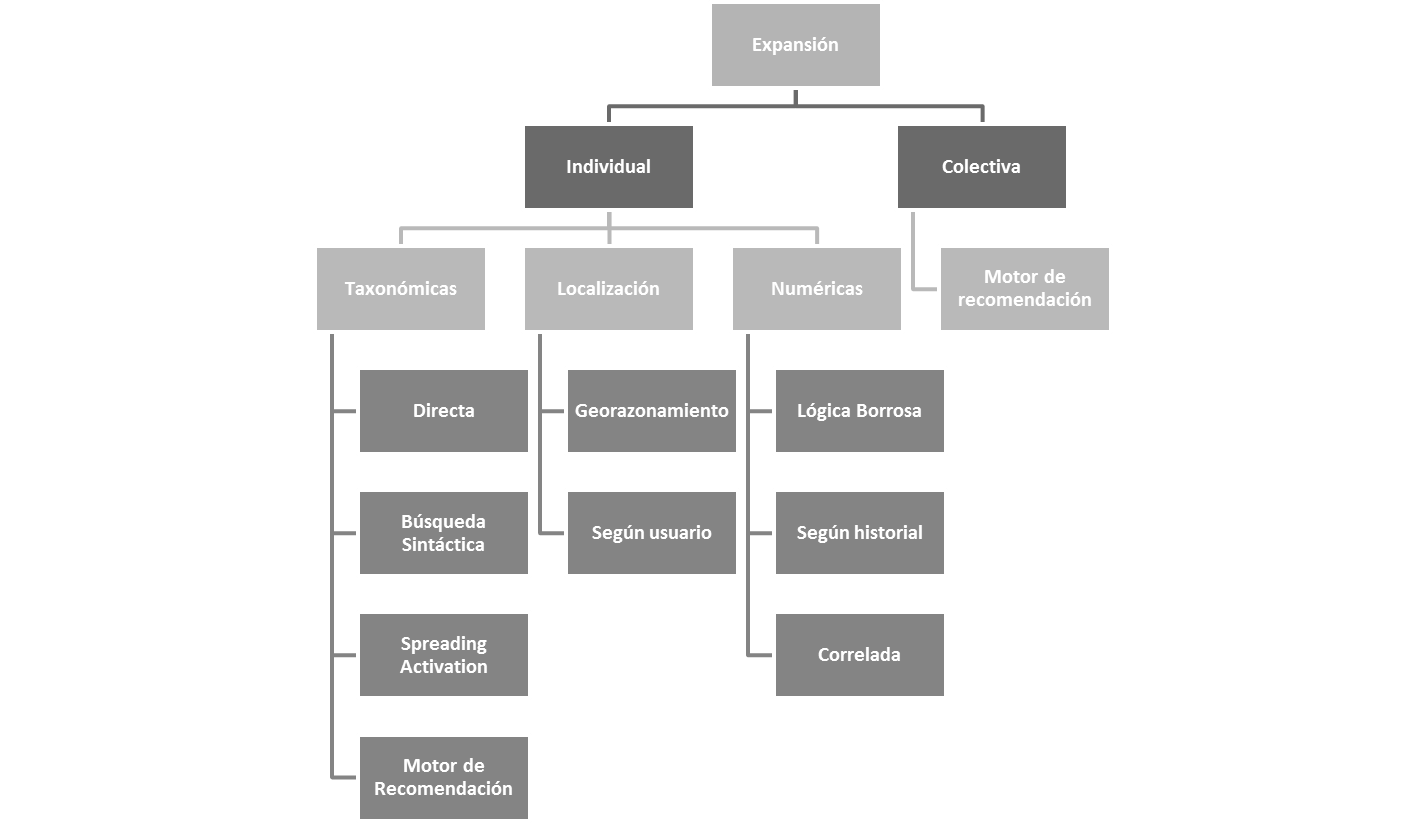
\includegraphics[width=9cm]{imgs/query-expansion}
% \caption{Métodos de Expansión de Consulta.}
% \end{figure}
% }
% 
% \frame{
%   \frametitle{Pruebas y Validación} 
% \begin{exampleblock}{Pruebas de Código Fuente}
%  \begin{itemize}
%  \item $140$ \textit{tests}.
%  \item $48$ clases Java específicas para Junit.
%  \item Métricas de código fuente de alta cohesión y bajo acoplamiento.
% \end{itemize}
% \end{exampleblock}
% }

\frame{
  \frametitle{MOLDEAS web (REST+Jquery)} 
\begin{figure}[!htb]
\centering
	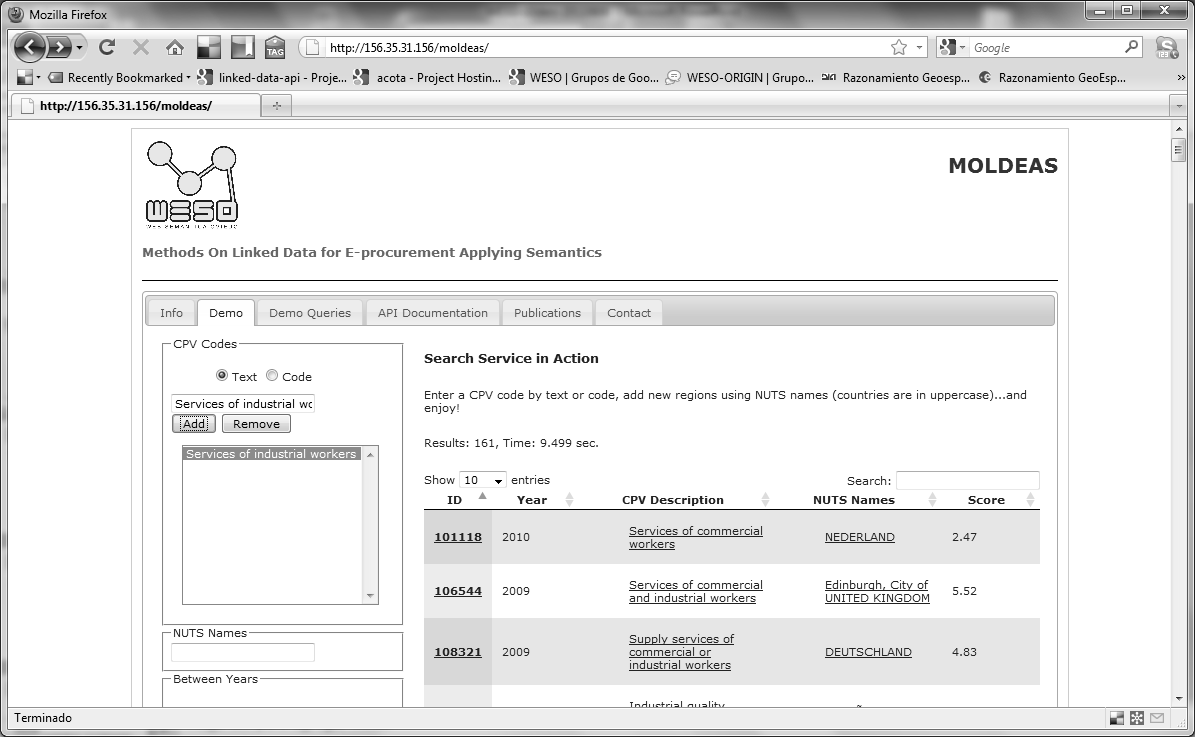
\includegraphics[width=10cm]{imgs/moldeas-web}
\end{figure}

}
\frame{
  \frametitle{MOLDEAS web-Resultados (Jquery+Exhibit)} 
\begin{figure}[!htb]
\centering
 	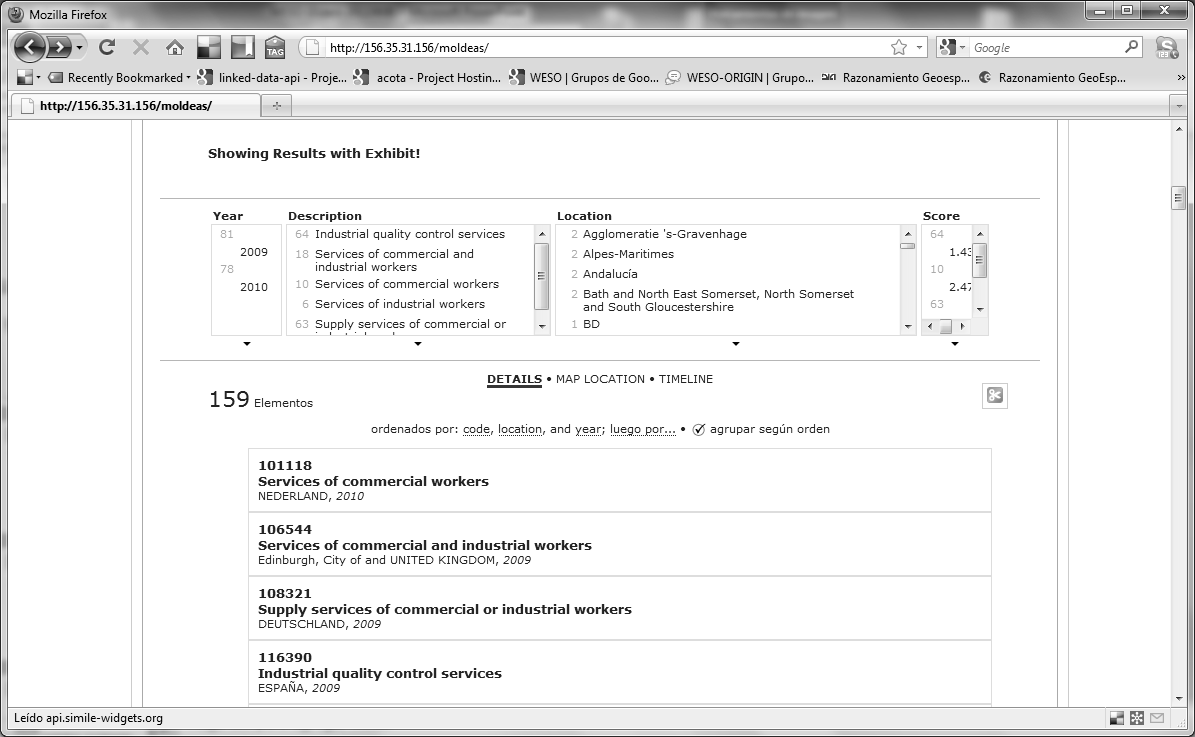
\includegraphics[width=10cm]{imgs/moldeas-results}

\end{figure}
}
\frame{
  \frametitle{MOLDEAS-Linked Data Frontend (Pubby)} 

\begin{figure}[!htb]
\centering
 	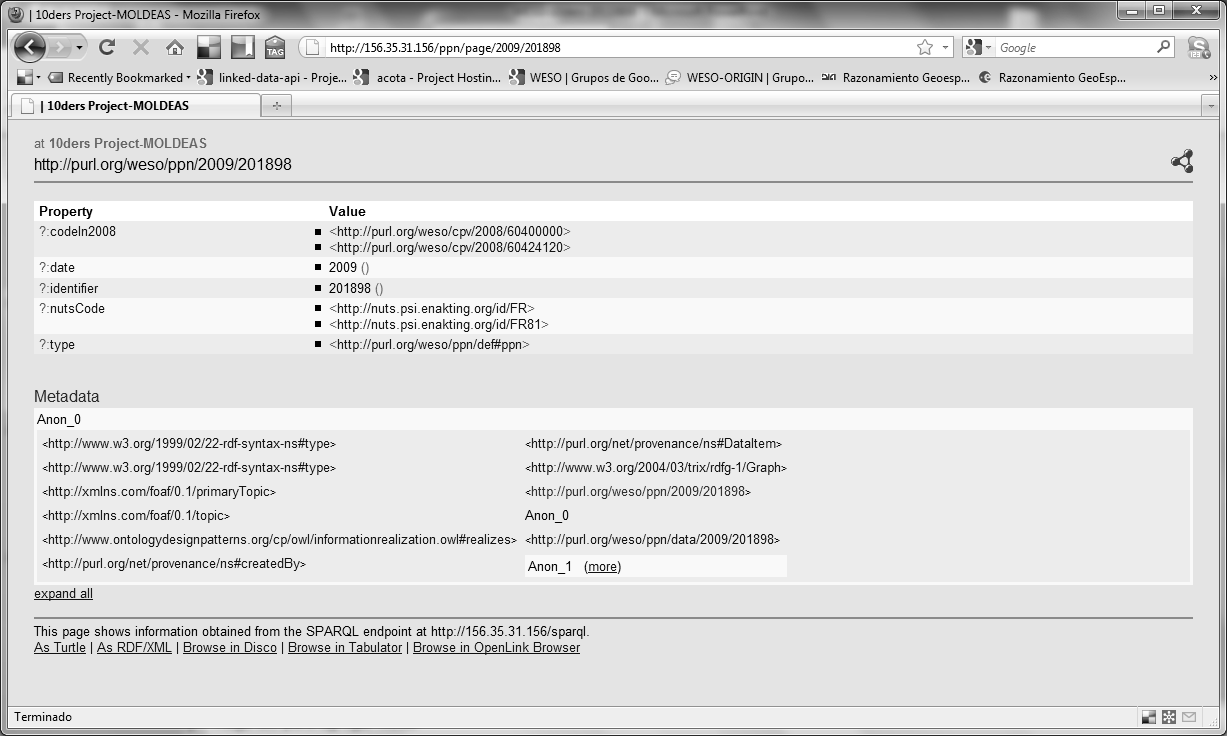
\includegraphics[width=10cm]{imgs/moldeas-pubby}

\end{figure}
}

% \frame{
%   \frametitle{MOLDEAS-Live queries (SNORQL)} 
% \begin{figure}[!htb]
% \centering
% 	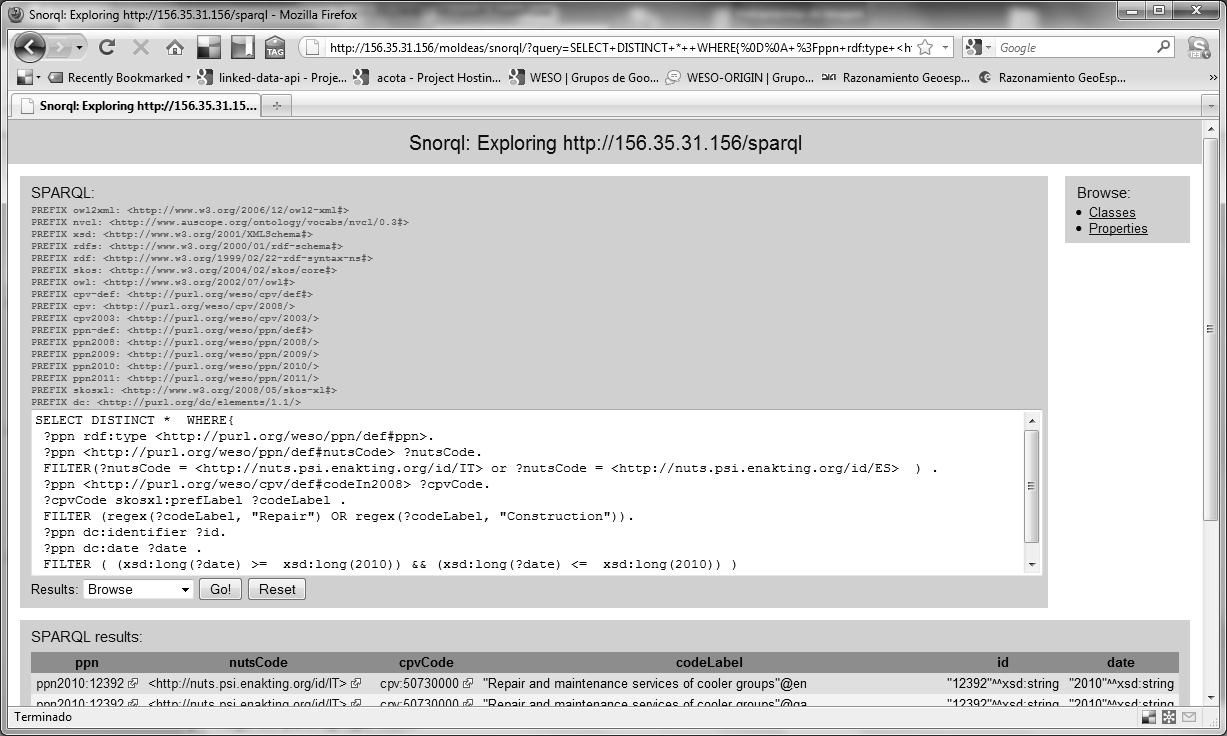
\includegraphics[width=10cm]{imgs/moldeas-snorql}
% \end{figure}
% 
% }
